%region LPR-Sentinel
\section{Sistema LPR-Sentinel}
LPR-Sentinel es un sistema de generación sintética, aumentación, detección y reconocimiento de matrículas para vehículos privados mexicanos, diseñado explícitamente para dar cumplimiento a los lineamientos establecidos en la primera versión de la NOM-001-SCT-2-2016. Esta norma, emitida por la Secretaría de Comunicaciones y Transportes (SCT), establece las especificaciones físicas, tipográficas y de seguridad que deben cumplir las placas de matrícula a nivel nacional.

Entre los aspectos más relevantes que regula la norma se encuentran las dimensiones oficiales de la placa (300 mm de ancho por 150 mm de alto), los colores y elementos de refracción según el tipo de vehículo y servicio, la tipografía de alto relieve para caracteres y números, así como la inclusión de elementos de seguridad como el Escudo Nacional, códigos bidimensionales y elementos ópticamente variables. Adicionalmente, la NOM-001-SCT-2-2016 define los diferentes tipos de matrículas atendiendo al servicio prestado: particulares, vehículos de gobierno, servicio público de pasajeros y carga, vehículos diplomáticos, autos antiguos y colección, así como matrículas para personas con discapacidad o vehículos motores de dos ruedas. Cada una de estas categorías cumple con combinaciones cromáticas y sistemas de identificación específicas. Para los vehículos particulares, actualmente la única clase compatible con nuestro sistema, la norma especifica la estructura alfanumérica LLL-NNN-L (L: letra, N: número) como el patrón general para la mayoría de las entidades federativas, con variaciones particulares para la Ciudad de México (LNN-LLL) y Guanajuato (LLL-NN-LL) previo a las actualizaciones de la norma. El alfabeto permitido excluye las letras \quotes{I}, \quotes{Ñ}, \quotes{O} y \quotes{Q} para evitar confusiones con los dígitos \quotes{1} (uno), \quotes{0} (cero) y \quotes{N}, empleando 33 caracteres posibles (incluyendo el guion \quotes{-} como separador).

Frente a esta diversidad de condiciones, el sistema propuesto adopta un enfoque basado en datos sintéticos, en lugar de depender de la recolección y etiquetado manual de imágenes reales. Esta decisión resuelve las complejidades éticas y legales asociadas al manejo de datos reales y garantiza el control absoluto sobre la distribución, variabilidad y anotación de los conjuntos de entrenamiento. La arquitectura, desglosada en cinco componentes funcionales independientes como se ilustra en la Figura \ref{fig_pipeline}, permite abordar de manera particular cada etapa del proceso de reconocimiento, desde la generación de muestras sintéticas hasta la consulta de información vehicular asociada. Esta modularidad facilita la evaluación aislada de cada componente y la mejora del sistema conforme sea necesario.

\begin{figure}[ht]
\centering
\includegraphics[width=0.8\textwidth]{figures/lpr_sentinel_pipeline.pdf}
\caption[Arquitectura general del sistema LPR-Sentinel]{Arquitectura general del sistema LPR-Sentinel. Las imágenes de entrada son procesadas secuencialmente por el módulo de detección (MLP-Detector), que localiza la región de la matrícula. Dicha región es recortada y enviada al módulo de reconocimiento (MLP-Recognizer), que extrae la cadena alfanumérica. Finalmente, el texto reconocido es consultado en una base de datos SQLite que retorna la información asociada al vehículo y su propietario. Los módulos de generación y aumentación de datos (no necesarios para el proceso de inferencia) proveen los conjuntos de entrenamiento solo para el módulo de detección y reconocimiento.}
\label{fig_pipeline}
\end{figure}
%endregion

%region MLP-Generator
\subsection*{MLP-Generator}
\addcontentsline{toc}{subsection}{MLP-Generator}
\textit{Mexican Licence Plate Generator} (MLP-Generator) es el motor de generación procedimental de matrículas mexicanas desarrollado conforme a la NOM-001-SCT-2-2016. Diseñado para crear bases de datos sintéticas que resuelvan las limitaciones éticas y legales del empleo de datos reales. Su funcionamiento requiere disponer de las 32 plantillas de matrículas estatales, nuestra fuente tipográfica de alto relieve pseudo-oficial y la parametrización del algoritmo para la producción de las series alfanuméricas válidas. Como resultado se obtiene un dataset sintético de matrículas ideales y una base de datos con información virtual asociada (propietario, tipo de vehículo, estado legal, entre otros atributos relacionados).

\subsubsection*{Arquitectura de generación basada en plantillas}
\addcontentsline{toc}{subsubsection}{Arquitectura de generación basada en plantillas}
El algoritmo opera bajo una arquitectura de generación basada en plantillas (\textit{template-based generation}), tomando como referencia una imagen de $500 \times 246$ píxeles por cada estado. Las plantillas han sido adaptadas de información pública \cite{matriculas-mexico} y manipuladas para asegurar el espacio editable de la serie. El módulo permite parametrizar la cantidad de matrículas a generar por estado, ya sea de manera global o por entidad específica, respetando los espacios destinados a los caracteres.

De acuerdo con la norma, los caracteres utilizados incluyen todos los guarismos numéricos (0-9) y las letras del alfabeto español excluyendo \quotes{I}, \quotes{Ñ}, \quotes{O} y \quotes{Q}, más el guion separador \quotes{-}, conformando el diccionario \mbox{\quotes{0123456789ABCDEFGHJKLMNPRSTUVWXYZ-}}. La selección de caracteres sigue los formatos LLL-NNN-L (mayoría de estados), LNN-LLL (Ciudad de México) y LLL-NN-LL (Guanajuato) mediante una estructura de datos que ajusta la longitud y tipo de carácter en cada posición. Además, se respetan los rangos exclusivos por estado (ej. Aguascalientes: AAA-AFZ, Zacatecas: ZDA-ZHZ) según el Apéndice C de la norma. La Figura \ref{fig_generacion_placas} ejemplifica algunos resultados de este proceso de generación sintético.

\begin{figure}[ht]
\centering
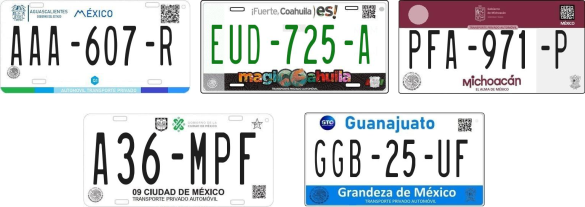
\includegraphics[width=0.65\textwidth]{figures/matriculas_sinteticas.png}
\caption[Ejemplos de matrículas sintéticas generadas por MLP-Generator]{Ejemplos de matrículas sintéticas generadas por MLP-Generator. Fila superior: Aguascalientes, Coahuila y Michoacán (formato LLL-NNN-L). Fila inferior: Ciudad de México (LNN-LLL) y Guanajuato (LLL-NN-LL).}
\label{fig_generacion_placas}
\end{figure}

\subsubsection*{\fontseries{sb}Diseño y construcción de la fuente tipográfica}
\addcontentsline{toc}{subsubsection}{Diseño y construcción de la fuente tipográfica}
Al no disponer de la fuente tipográfica oficial, se diseñó una fuente de autoría propia respetando las cotas indicadas en el documento normativo. Cada carácter se dibujó manualmente con el software de dibujo vectorial Inkscape \cite{inkscape}, respetando curvas, longitudes, grosores y colores. Los caracteres se integraron en una fuente única usando FontForge \cite{fontforge}, generando un archivo TTF cuyo diccionario se ilustra en la Figura \ref{fig_fuente_TTF}.

\begin{figure}[ht]
\centering
\includegraphics[width=0.5\textwidth]{figures/fig_fuente_TTF.pdf}
\caption[Diccionario de la fuente tipográfica]{Diccionario de la fuente tipográfica diseñada, que incluye los 33 caracteres permitidos por la NOM-001-SCT-2-2016 (dígitos 0-9, letras mayúsculas excluyendo I, Ñ, O, Q, y el guion). Las cotas dimensionales se expresan en milímetros.}
\label{fig_fuente_TTF}
\end{figure}

\subsubsection*{Parametrización del generador}
\addcontentsline{toc}{subsubsection}{Parametrización del generador}
MLP-Generator es un módulo externo al pipeline del sistema LPR-Sentinel. Fue diseñado con el lenguaje de programación Python destinado a manipularse a través de la interfaz de línea de comandos (CLI). Este módulo permite al usuario parametrizar la cantidad de matrículas a generar por estado global o para una entidad federativa específica, funcionalidad que permite equilibrar \textit{datasets} en entrenamientos específicos o replicar el procedimiento bajo distintas condiciones. El programa separa la lógica de validación de la lógica de selección de caracteres, asegurando que la salida no sea únicamente una cadena aleatoria, sino un registro que podría existir legalmente dentro del sistema nacional de matriculación. A diferencia de los algoritmos de generación criptográfica, donde la impredecibilidad absoluta constituye el objetivo, este generador persigue la predictibilidad normativa. Esto significa que la aleatoriedad está contenida dentro de los rangos permitidos por el Apéndice C de la norma, el cual detalla las series asignadas para evitar duplicados nacionales. El programa modela matemáticamente estos rangos, permitiendo la generación de secuencias que respetan las fronteras de las series estatales, como la transición de AAA a AFZ para el mismo estado de Aguascalientes del ejemplo previo. Esta capacidad de replicar la distribución real de las matrículas es lo que otorga valor científico a la herramienta, ya que permite simular escenarios de tráfico con una fidelidad estadística que los modelos puramente aleatorios no podrían alcanzar.

Paralelamente a cada generación de matrícula se sintetizan los datos virtuales necesarios para simular una base de datos utilizable con fines didácticos de seguridad. Información como el nombre del propietario de la matrícula, la marca, el modelo y el color del vehículo asociado, la entidad federativa de registro y el estado legal del vehículo, así como la fecha de registro, son generados de manera pseudoaleatoria, siendo todos ellos creados de forma procedimental mediante la definición de diferentes conjuntos de características y operados como producto cartesiano de la forma $A \times B \times C$ para la generación extensa y sin duplicación de cada matrícula. Siendo esta base de datos una primera aproximación a un sistema completo de verificación de matrículas.

Al contrastar nuestra propuesta de generación sintética de matrículas con las existentes en la literatura académica actual, se observa como distinción la creación de imágenes de matrículas que no solo contienen la cadena de texto, sino también las texturas propias de la placa metálica. Sin embargo, aunque esta solución genera matrículas que garantizan el cumplimiento de la norma, no resulta suficiente para representar las condiciones del mundo real, volviéndose indispensable la aplicación de transformaciones morfológicas y filtros que simulen las condiciones reales que aporten este realismo a las imágenes.
%endregion
    
%region MLP-Augmentator
\subsection*{MLP-Augmentator}
\addcontentsline{toc}{subsection}{MLP-Augmentator}
Los sistemas ALPR y OCR dependen de la diversidad y el volumen de los conjuntos de datos utilizados durante el entrenamiento. La variabilidad de las condiciones ambientales, los ángulos de captura y las degradaciones físicas de las matrículas es un desafío que no puede ser cubierto exclusivamente mediante la generación de datos sintéticos ideales, por lo que el dataset generado por el módulo MLP-Generator no es suficiente. \textit{Mexican Licence Plate Augmentator} (MLP-Augmentator) aborda esta problemática mediante un proceso de aumentación de los datos donde se transforman las imágenes base de matrículas generadas en miles de variantes sintéticas. Nuestra herramienta implementa 29 aumentaciones integradas por transformaciones geométricas, degradaciones ópticas y ajustes fotométricos adaptados de \cite{albumentations}, diseñados de forma equivalente usando la librería OpenCV con la intención de evitar pagos o uso de librerías privadas de terceros. La Tabla \ref{tab_transforms} presenta un resumen de todas las transformaciones disponibles en nuestro sistema.
\vspace{0.7 cm}

\sffamily
\footnotesize
\refstepcounter{table}
\begin{tcolorbox}[
  colback=white,
  colframe=MASA-Blue,
  title={Tabla~\thetable~Transformaciones implementadas en el módulo MLP-Augmentator},
  boxrule=0.5mm,
  arc=2mm,
  width=\textwidth,
  enhanced,
  fonttitle=\bfseries,
  before upper=\vspace{2mm},
  after upper=\vspace{2mm}
]
\label{tab_transforms}
\renewcommand{\arraystretch}{1.5}
\begin{tabularx}{\textwidth}{@{}l X@{}}
\textbf{Transformación} & \textbf{Descripción} \\
\midrule
Motion blur & Simula desenfoque por movimiento con diferentes umbrales de intensidad \\
Auto contrast & Altera el contraste automáticamente \\
Defocus blur & Simula el desenfoque de la cámara \\
Color jitter & Altera el brillo, contraste y saturación aleatoriamente \\
Channel dropout & Elimina aleatoriamente un canal de color \\
Dithering & Reduce la profundidad de color creando un efecto de difuminado \\
Downscale (0.25, 0.5, 0.75) & Simula baja resolución mediante submuestreo y reescalado \\
Equalize & Aplica ecualización de histograma con el algoritmo CLAHE \\
Glass blur & Simula visión a través de vidrio distorsionado \\
ISO noise & Añade ruido aleatorio simulando alta sensibilidad ISO \\
Illumination & Simula diferentes condiciones de iluminación diurna y nocturna \\
Random fog & Añade efecto de niebla \\
Random occlusion & Añade oclusiones aleatorias \\
Random rain & Simula la presencia de lluvia \\
Random shadow & Añade sombras aleatorias \\
Random snow & Simula la presencia de partículas de nieve \\
Random sun flare & Simula destellos solares \\
Spatter & Simula salpicaduras de barro o agua \\
Rotation (25, 50, 75) & Rota la imagen en ángulos específicos sobre el plano XY \\
Scale (0.25, 0.5, 0.75) & Escala la imagen manteniendo la relación de aspecto \\
Perspective (0.35, 0.5, 0.7) & Aplica distorsión de perspectiva controlada sobre el espacio XYZ \\
\end{tabularx}
\end{tcolorbox}
\normalsize
\normalfont
\newpage

\subsubsection*{Aumentación geométrica}
\addcontentsline{toc}{subsubsection}{Aumentación geométrica}
El programa, también programado empleando el lenguaje Python, implementa una lógica de transformación de perspectiva que permite alterar el dataset ideal y dotarlo de escenarios posibles en el mundo real. Uno de estos escenarios es la presencia de inclinación frontal y lateral que representan ángulos de visión extremos capturados por una cámara. Mediante el uso de OpenCV, se calculan las matrices de transformación $M$ aplicada a los cuatro vértices de la imagen original, correspondientes a las esquinas de una placa asumiendo que su captura se realiza desde un plano frontal, y se proyecta la matrícula en un espacio tridimensional virtual que simula estos escenarios donde pudo haber sido capturada desde distintos ángulos. Este enfoque supera las rotaciones bidimensionales simples al modelar la deformación trapezoidal presente en las capturas laterales o elevadas, obligando al modelo de aprendizaje a aprender características invariantes de la fuente tipográfica en lugar de formas rígidas e ideales. Complementando la perspectiva, la lógica de rotación integrada en el sistema destaca por recalcular dinámicamente el contenedor de la imagen para evitar el truncamiento de los caracteres. Esta implementación asegura que la integridad visual de la placa se mantiene intacta, permitiendo rotaciones desde 25 grados, típicas en vehículos en movimiento o cámaras desalineadas, hasta 75 grados, que simularían un punto crítico de captura, como el desajuste o caída de la cámara.% Asimismo, la función de redimensión con preservación de la relación de aspecto y relleno de bordes garantiza que las muestras finales cumplan con las dimensiones de entrada requeridas por las arquitecturas de visión actuales sin deformar las proporciones legales de la matrícula.

\subsubsection*{Aumentación óptica y de ruido ambiental}
\addcontentsline{toc}{subsubsection}{Aumentación óptica y de ruido ambiental}
Otro de los principales problemas en la captura de placas vehiculares es el desenfoque por movimiento o la baja resolución de los sensores. El programa también aborda estas limitaciones mediante un conjunto de algoritmos de degradación óptica que imitan condiciones reales de operación. La implementación de \texttt{motion blur} permite simular el desplazamiento lineal de un vehículo a alta velocidad, por ejemplo. Adicionalmente, el script introduce una degradación por submuestreo (\texttt{downscale}) que reduce la resolución de la imagen y la restaura mediante interpolación, generando el efecto de pixelación característico de las cámaras de vigilancia de bajo costo o de las transmisiones comprimidas. Para simular condiciones climáticas como la lluvia intensa o la visión a través de superficies distorsionadas, el script emplea una técnica de \texttt{glass blur}. Esta función desplaza píxeles individuales de forma iterativa basándose en un desplazamiento aleatorio limitado, creando una distorsión visual que preserva la estructura global de los caracteres, pero desafía la capacidad de segmentación del modelo.

Similarmente, la variabilidad lumínica, desde la exposición solar directa hasta la iluminación artificial nocturna, se simula aplicando variaciones aleatorias de brillo, contraste y saturación. Esta operación obliga a priorizar el reconocimiento de formas, bordes y gradientes en lugar de depender de firmas cromáticas específicas, lo cual es fundamental considerando que la norma NOM-001-SCT-2-2016 define colores particulares que pueden verse alterados por filtros de cámara o condiciones de sombra. % La mejora del contraste local se maneja mediante la técnica de Ecualización de Histograma Adaptativa Limitada por Contraste (CLAHE). El script realiza una conversión del espacio de color BGR al espacio LAB, aplicando CLAHE exclusivamente sobre el canal \quotes{L} (Lightness) antes de revertir la conversión. Este proceso permite resaltar los detalles de los caracteres troquelados en alto relieve de la placa mexicana sin introducir los artefactos de ruido que genera una ecualización global, mejorando la legibilidad en condiciones de subexposición o sobreexposición. 
Finalmente, el uso de técnicas de reducción de profundidad de bits simula la compresión digital agresiva, preparando al modelo para procesar transmisiones de video en tiempo real donde el ancho de banda se asume es limitado.

Estas degradaciones tampoco son meramente cosméticas. Investigaciones académicas han demostrado que el entrenamiento con imágenes con ruido inducido mejora la precisión de validación en entornos reales del 30\% al 78\% en condiciones de desenfoque severo. Al integrar estos efectos de forma estocástica, el módulo genera un dataset que previene el sobreajuste a imágenes de alta calidad. Aunque esta propuesta se rige por el uso de conjuntos de datos completamente sintéticos, abre la oportunidad de contrastar los resultados obtenidos contra conjuntos de datos reales y verificar si el aporte es significativo para futuras implementaciones.

Cabe mencionar que este segundo módulo es también parametrizable y toma como referencia cada imagen generada por el módulo MLP-Generator, creando una variante distinta con cada una de las transformaciones disponibles aplicadas de manera independiente para, posteriormente, someter a evaluación aquellas transformaciones más representativas en el sistema. Asimismo, es posible especificar la cantidad de variantes aplicadas, así como el tamaño de la imagen final, para reducir el tiempo de postprocesamiento previo al ingreso de nuestro modelo de reconocimiento OCR.
%endregion

%region MLP-Detector
\subsection*{MLP-Detector}
\addcontentsline{toc}{subsection}{MLP-Detector}
\textit{Mexican Licence Plate Detector} (MLP-Detector) es el módulo que constituye la primera etapa del pipeline de reconocimiento automático de placas. Se encarga de localizar la región de interés (ROI) correspondiente a la matrícula vehicular dentro de una imagen de mayor escala, como las capturadas por cámaras de vigilancia o dispositivos móviles en entornos no controlados. Como se ilustra en la Figura \ref{fig_detector}, este detector ha sido diseñado para procesar imágenes completas que pueden contener vehículos, fondos complejos, múltiples objetos y variaciones significativas de iluminación y perspectiva. La arquitectura seleccionada para esta tarea fue una Red Neuronal Convolucional basada en YOLO (You Only Look Once).% La elección de YOLO responde a la necesidad de integrar el detector en sistemas que requieren latencias reducidas, como cámaras de peaje, acceso a estacionamientos o patrullajes móviles, donde el procesamiento debe realizarse a velocidades de al menos 30 fotogramas por segundo.

\begin{figure}[ht]
\centering
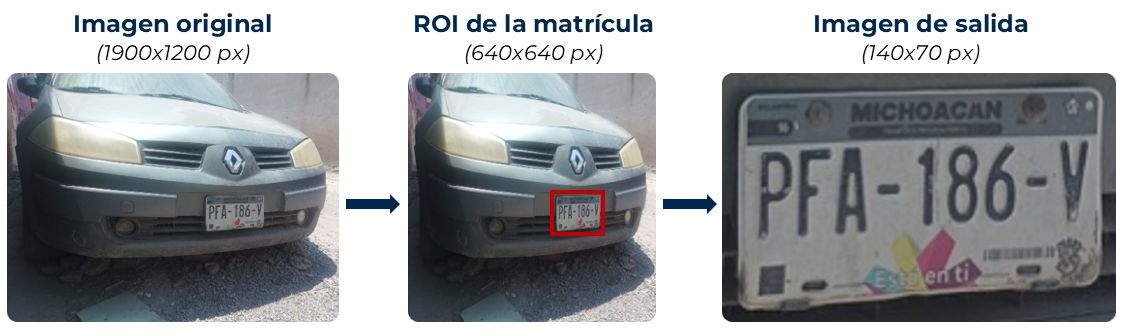
\includegraphics[width=0.85\textwidth]{figures/flujo_detector.png}
\caption[Flujo de operación del módulo MLP-Detector]{Flujo de operación del módulo MLP-Detector. El módulo recibe una imagen completa ($1900\times 1200$ px, por ejemplo), escala la imagen original a una dimensión de $640\times 640$ px y regresa la región de interés (ROI) donde se encuentra la placa vehicular con un tamaño de $140\times 70$ px.}
\label{fig_detector}
\end{figure}

El entrenamiento del modelo se realizó utilizando el framework PyTorch para la gestión del conjunto de datos y la aumentación de las muestras. El script de entrenamiento disponible como anexo al presente documento, indica el procedimiento de entrenamiento completo. El modelo base para la detección seleccionado fue YOLOv11s, correspondiente a la variante \quotes{small} de YOLOv11, que ofrece un equilibrio adecuado entre número de parámetros (aproximadamente 9 millones) y precisión media promedio (mAP) comparada con versiones previas y posteriores en \cite{jiang-zhong2025}, cuyo resultado promete ser suficiente para el despliegue en dispositivos con recursos limitados como la Raspberry Pi o cámaras IP con capacidades de procesamiento embebido.

Por limitaciones de hardware, el entrenamiento se realizó con 14 épocas y un tamaño de imagen de entrada de $640\times 640$ píxeles como prueba de concepto, dimensión estándar en la familia YOLO que permite capturar suficiente detalle contextual para la detección de patrones sin incurrir en un costo computacional excesivo. El conjunto de datos utilizado contiene imágenes de vehículos capturadas en diversas condiciones ambientales, ángulos de cámara y distancias, con anotaciones manuales que delimitan la posición de las matrículas mediante cajas delimitadoras rectangulares. Durante el proceso de entrenamiento, el modelo optimiza una función de pérdida compuesta que combina el error de localización de las cajas (utilizando pérdida CIoU, \textit{Complete Intersection over Union}), la pérdida de confianza por objeto y la pérdida de clasificación para distinguir la clase \quotes{placa} de cualquier otro objeto presente en la escena. Al finalizar las 14 épocas, los pesos del mejor modelo generado durante estas épocas, aquellos que maximizan la métrica mAP sobre el conjunto de validación, se almacenan en un archivo de PyTorch dentro del directorio de entrenamiento correspondiente.

Sin embargo, este modelo generado requiere el mismo framework de entrenamiento utilizado para las actividades de inferencia. Con la intención de separar el framework de entrenamiento con el entorno de inferencia, en nuestra solución se exporta el modelo entrenado al formato ONNX, un formato abierto que permite representar modelos de aprendizaje automático y profundo de manera estándar. El archivo ONNX resultante contiene un grafo computacional estático que puede ser ejecutado por cualquier motor de inferencia compatible, incluyendo OpenCV DNN, TensorRT (especialmente optimizado para GPUs NVIDIA) o ONNX Runtime, siendo este último el motor de inferencia seleccionado para su ejecución sobre nuestra propuesta de sistema embebido.

La inferencia del detector realiza el flujo completo de procesamiento desde la imagen de entrada hasta la extracción de la región de la placa, sin aún reconocer los caracteres presentes en ella. El proceso comienza con la carga de la imagen mediante OpenCV y el almacenamiento de sus dimensiones originales, información necesaria para la posterior transformación de coordenadas. La imagen es redimensionada a $640\times 640$ píxeles, el tamaño esperado por el modelo, y sus píxeles son convertidos al tipo \texttt{float32} y normalizados al rango [0,1] mediante la división por 255, una práctica común en YOLO durante el preprocesamiento. La imagen normalizada es entonces transpuesta para cambiar el orden de las dimensiones de (alto,ancho,canales) a (canales,alto,ancho), formato requerido por el motor de inferencia ONNX Runtime para las entradas de tipo imagen.

La salida del modelo YOLO en ONNX tiene una forma característica: (1,84,8400) para una imagen de entrada de $640 \times 640$. El número 84 corresponde a 4 coordenadas de la caja delimitadora (x,y,ancho,alto) más 80 probabilidades de clase, aunque en este caso particular solo se utiliza una clase efectiva (matrícula), manteniéndose la estructura estándar por compatibilidad. El valor 8400 representa el número total de predicciones generadas por el modelo en diferentes escalas y posiciones de la cuadrícula. El script implementa una función de postprocesamiento que transforma esta salida en cajas delimitadoras interpretables. Primero, se extrae la matriz de predicciones y se transpone para obtener una estructura de (8400,84). Se aplica una máscara de confianza que filtra aquellas predicciones cuya probabilidad de clase máxima supera el umbral establecido en 0.7 (70\%), valor seleccionado empíricamente para equilibrar la sensibilidad en entornos de prueba. Las coordenadas de las cajas, originalmente expresadas como (x(centro), y(centro), ancho, alto) en el espacio normalizado de $640\times 640$, son convertidas al formato (x1,y1,x2,y2) y escaladas a las dimensiones originales de la imagen mediante factores de escala.

%Para eliminar detecciones redundantes que corresponden al mismo objeto, el script aplica el algoritmo Non-Maximum Suppression (NMS). Este algoritmo selecciona la caja con mayor confianza dentro de un conjunto de detecciones solapadas, suprimiendo aquellas cuyo solapamiento, medido mediante Intersection over Union (IoU), supera el umbral de 0.45. 
Las cajas resultantes representan las detecciones finales de matrículas en la imagen original. Sobre cada detección que corresponde a la clase 0 (matrícula) y cuyo filtro de confianza excede el 70\%, el script extrae la región de interés aplicando un margen de 5 píxeles en cada dirección, expansión que permite incluir contexto adicional alrededor de la placa y así facilitar el trabajo del módulo reconocedor siguiente. Esta región recortada se almacena temporalmente en un directorio de salida, mientras que la imagen original se dibuja con el rectángulo delimitador y la etiqueta de confianza con la que se infiere existe una placa.%, redimensionándose posteriormente a un ancho de 720 píxeles mediante una función de escala para su visualización y almacenamiento.% El tiempo de inferencia se mide y reporta, proporcionando una métrica cuantitativa del rendimiento del detector en el hardware de despliegue.
%endregion

%region MLP-Recognizer
\subsection*{MLP-Recognizer}
\addcontentsline{toc}{subsection}{MLP-Recognizer}
\textit{Mexican Licence Plate Recognizer} (MLP-Recognizer) es el componente central de inferencia del sistema propuesto. Este módulo es el encargado de reconocer los carácteres de las áreas de interés detectadas por el módulo MLP-Detector, ya sean de imágenes sintéticas o reales. Este reconocedor ha sido diseñado para operar en entornos de producción con restricciones de latencia y recursos computacionales, también empleando para ello el formato ONNX como interfaz de despliegue.

La arquitectura del reconocedor se basa en un modelo de tipo CCT (Compact Convolutional Transformer), cuya configuración se encuentra documentada en \cite{fastplateOCR}. Este modelo combina las ventajas de las capas convolucionales para la extracción de características locales con la capacidad de los Vision Transformers para modelar dependencias secuenciales a larga distancia. El modelo requiere trabajar con imágenes de 70 píxeles de alto por 140 de ancho, por lo que imágenes con una dimensión diferente es escalada manteniendo la relación de aspecto original mediante la técnica de \textit{letterboxing}, un algoritmo que centra la imagen sobre un fondo negro cuando la imagen de entrada tiene una dimensión inferior a la esperada sin que se desee alterar la información original. El modo de color empleado es escala de grises, reduciendo así la dimensionalidad de los datos de entrada a un único canal. Una vez redimensionada, la imagen es convertida al tipo \texttt{float32} y presentada al modelo sin normalización adicional.

El modelo produce una salida con forma (1,9,33), donde 9 corresponde al número máximo de posibles caracteres que puede contener una matrícula mexicana conforme al formato estándar LLL-NNN-L y sus variantes estatales, y 33 representa el tamaño del diccionario definido en la configuración de entrenamiento. El carácter de relleno, también definido como \quotes{-}, se utiliza para completar aquellas placas cuya longitud efectiva es inferior a nueve caracteres, garantizando que todas las salidas mantengan una dimensionalidad común. La decodificación de la predicción se realiza aplicando la función softmax sobre las activaciones de cada caracter, seleccionando el índice con mayor probabilidad y mapeándolo al carácter correspondiente en el diccionario. El script de inferencia calcula además la confianza por cada posición como la probabilidad asignada al carácter elegido, proporcionando así una métrica de fiabilidad que permite filtrar predicciones dudosas o activar mecanismos de reintento (no implementados en esta primera versión).

El proceso de inferencia se implementa sobre una interfaz de línea de comandos parametrizable. Este script replica exactamente el preprocesamiento utilizado durante el entrenamiento del modelo original en Tensorflow, condición indispensable para garantizar la coherencia entre las fases de aprendizaje y despliegue. Inicialmente se carga la imagen mediante OpenCV, se convierte a escala de grises, y aplica el redimensionamiento con preservación de la relación de aspecto utilizando interpolación lineal.

%Entre las capas más relevantes de la arquitectura empleada destacan \texttt{MaxBlurPooling2D}, que combina operaciones de agrupamiento con filtros de suavizado para reducir la pérdida de información en el submuestreo. \texttt{PatchExtractor} y \texttt{PositionEmbedding}, que segmentan la imagen en parches y añaden información posicional. \texttt{TransformerBlock} y \texttt{TokenReducer}, que implementan la mecánica de atención con reducción progresiva de tokens para mejorar la eficiencia computacional y \texttt{VocabularyProjection}, que proyecta las representaciones al espacio del vocabulario de salida. Por compatibilidad, la exportación requiere parchear la función de activación GELU (\textit{Gaussian Error Linear Unit}) para evitar el uso de operaciones no soportadas por ONNX, reemplazándola por una aproximación basada en la función tangente hiperbólica que preserva la fidelidad numérica mientras asegura la compatibilidad multiplataforma. 
El proceso de conversión genera un archivo ONNX que contiene tanto la estructura del grafo computacional como los pesos entrenados, todo ello en un formato estándar que puede ser consumido por cualquier motor de inferencia compatible.
%endregion

%region MLP-Pipeline
\subsection*{MLP-Pipeline}
\addcontentsline{toc}{subsection}{MLP-Pipeline}
\textit{Mexican Licence Plate Pipeline} (MLP-Pipeline) constituye la capa de integración de todo el sistema de reconocimiento LPR-Sentinel, coordinando la interacción secuencial entre el detector, el reconocedor óptico de caracteres y una base de datos de registro vehicular. Este módulo ha sido diseñado como un módulo cohesivo, el cual encapsula toda la lógica necesaria para transformar una imagen de escena completa en información estructurada sobre el vehículo y su propietario, ofreciendo una interfaz unificada que abstrae la complejidad de los modelos ONNX, los preprocesamientos específicos y las consultas a la base de datos.

La arquitectura del pipeline inicializa todos los componentes necesarios durante su construcción. Para su funcionamiento requiere los modelos ONNX del detector y del reconocedor, un archivo de configuración YAML de la arquitectura empleada en el modelo OCR, la ubicación de la base de datos y un directorio de salida para los resultados generados. Internamente, el módulo carga los modelos mediante el motor de inferencia ONNX Runtime, preconfigurado con el archivo de configuración del reconocedor que describe el diccionario empleado, las dimensiones de entrada de la imagen y el modo de color (escala de grises). Posteriormente establece la conexión con una base de datos local SQLite, la cual contiene la información sintética sobre la matrícula, el estado de registro, la marca y modelo del vehículo, el color, el estatus legal, el propietario y la fecha de registro, misma que fue generada durante la fase de creación del dataset desde el módulo MLP-Generator.

MLP-Pipeline sigue entonces la siguiente secuencia de etapas: (i) carga de imagen/frame y detección de la placa, (ii) extracción de la región de interés, (iii) reconocimiento óptico de caracteres y (iv) consulta a la base de datos. En la primera etapa, se carga la imagen mediante OpenCV, se redimensiona a $640\times 640$ píxeles, normaliza sus valores al rango [0,1] mediante división por 255 y transpone las dimensiones al formato de canales con el que fue entrenado. El tensor generado es pasado al modelo YOLO previamente cargado, y a las salidas obtenidas se les aplica un filtrado por umbral de confianza (0.7, para reportar solo aquellas inferencias que tienen un 70\% de certeza). Si la detección correspondiente a la clase 0 (matrícula vehicular) es exitosa, entonces se retorna la región de interés.

Una vez localizada la placa, el pipeline procede a la extracción de la ROI aplicando un margen de 5 píxeles en cada dirección, expansión que permite incluir un pequeño contexto alrededor de la matrícula y así mitigar posibles errores de delimitación del detector. Esta región recortada es almacenada en el directorio de salida con un nombre derivado del archivo original, y simultáneamente se dibuja sobre la imagen original el rectángulo delimitador junto con la etiqueta de confianza, generándose una imagen de visualización completa que facilita la depuración y la presentación de resultados. La tercera etapa corresponde al reconocimiento OCR, para lo cual la ROI es procesada aplicando una conversión a escala de grises, redimensionamiento a $70 \times 140$ píxeles con preservación de la relación de aspecto sobre un canvas negro en caso de ser necesario, y conversión a \texttt{float32} sin normalización adicional, dado que el modelo incorpora una capa de escalado por 1/255 por defecto. El tensor resultante es alimentado al modelo ONNX del reconocedor, y la salida con forma (1,9,33) es decodificada mediante nuestra función de inferencia, que selecciona el carácter con máxima probabilidad para cada posición, y calcula la confianza individual por carácter así como la confianza promedio de toda la matrícula.

La cuarta y última etapa del pipeline consiste en la consulta a la base de datos SQLite utilizando el texto de la placa reconocida como clave primaria. El módulo ejecuta una sentencia SELECT sobre nuestra tabla sintetica de registros y, si existe un registro con esa matrícula, retorna un diccionario con todos los campos asociados, incluyendo el nombre del propietario, el estado de procedencia, el estatus legal (por ejemplo, \quotes{regular}, \quotes{robado} o \quotes{reportado}), y la fecha de registro, entre otros, en caso contrario, se retorna un mensaje de advertencia.
%endregion